\section{Results}
\label{sec:results}

We first describe the distribution of crowd judgments and revisit the
majority--minority reception pattern as a baseline. We then examine the
reception of blaming and defending dissent in AITA (RQ1), their prevalence
over time (RQ2), and the extension to AITAH (RQ3). Figures that contain both
communities are discussed first for AITA and revisited in the community
comparison.

\subsection{Descriptive Context: Agreement and Verdict Stability}
\label{subsec:res-distribution}

The high-volume cohort comprises $28{,}107$ AITA and $8{,}217$ AITAH posts.
The distribution of YA share is sharply bimodal, with a larger concentration
near unanimous NA judgments than near unanimous YA judgments
(Figure~\ref{fig:ya-share}). High-agreement posts account for $78.2\%$ of
AITA and $81.6\%$ of AITAH posts, compared with $6.5\%$ and $4.7\%$ for
low-agreement posts. NA is dominant in $75.7\%$ and $87.4\%$ of posts,
respectively. High-agreement posts therefore constitute the larger
analytical condition, while NA-dominant and YA-dominant contexts differ
substantially in frequency. Detailed verdict and minority-share distributions
are reported in Appendix~\ref{sec:appendix-verdict-distribution}
(Table~\ref{tab:verdict-distribution}).

\begin{figure*}[t]
  \centering
  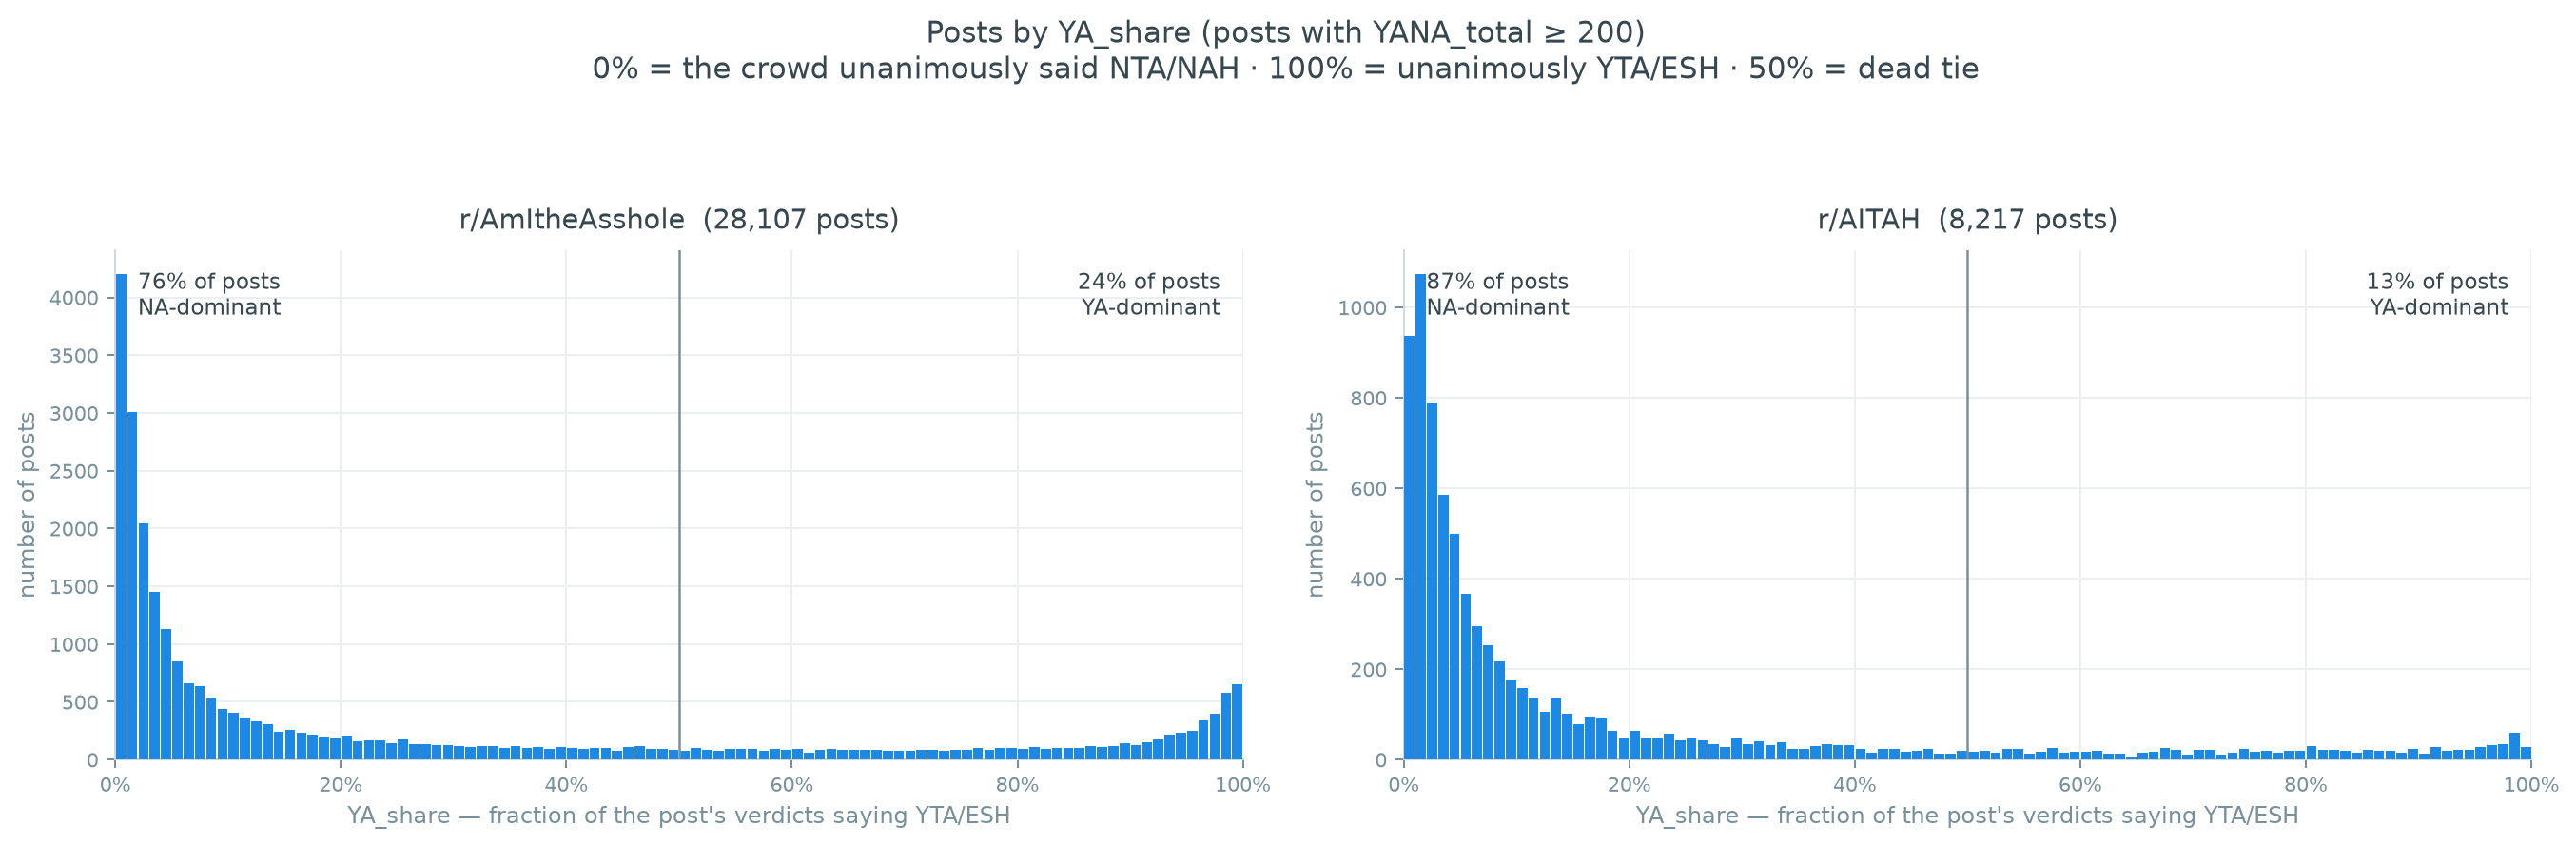
\includegraphics[width=\textwidth]{figures/ya_share_distribution.png}
  \caption{Distribution of posts by final YA share $\rho(p)$ over the
  high-volume cohort. The axis label \texttt{YA\_share} denotes $\rho(p)$,
  displayed as a percentage. A share of $0$ means the crowd unanimously exculpated the OP, $1$
  that it unanimously blamed them, and $0.5$ a dead tie. Both communities are
  sharply bimodal with an almost empty middle, and the two modes are far from
  symmetric: the exculpating peak is much the larger, especially in AITAH.}
  \label{fig:ya-share}
\end{figure*}

In high-agreement posts, early verdict leaders more often match the final
dominant judgment than in low-agreement posts
(Appendix~\ref{sec:appendix-stabilization},
Figure~\ref{fig:consensus-stabilization}). This correspondence does not
establish the opinion climate perceived by individual commenters.

\subsection{Baseline: Majority--Minority Reception Across Agreement Levels}
\label{subsec:res-baseline}

We revisit the score--reply pattern as a baseline rather than a separate
research question. In high-agreement AITA posts, majority and minority
comments have mean scores of $37.95$ and $-2.75$, respectively, while their
mean direct-reply counts are $0.14$ and $0.53$
(Figure~\ref{fig:engagement-by-consensus}). In low-agreement posts, the score
gap is smaller and the mean reply counts are closer: $0.26$ for majority
and $0.30$ for minority comments. The AITAH comparison is reported under RQ3.

\begin{figure}[t]
    \centering
    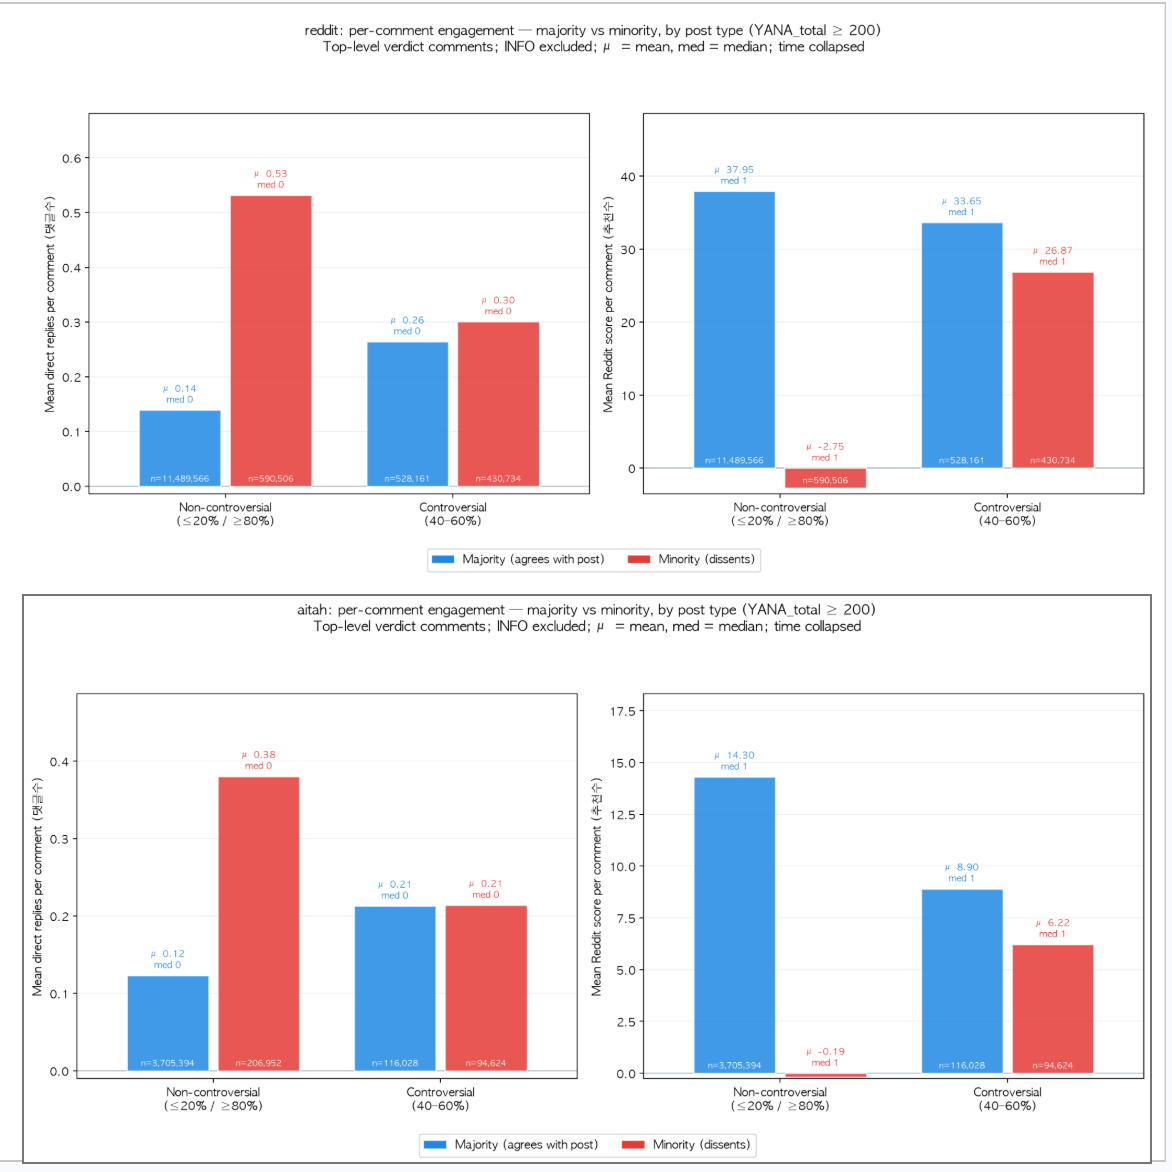
\includegraphics[width=\columnwidth]
    {figures/engagement_by_consensus.png}

    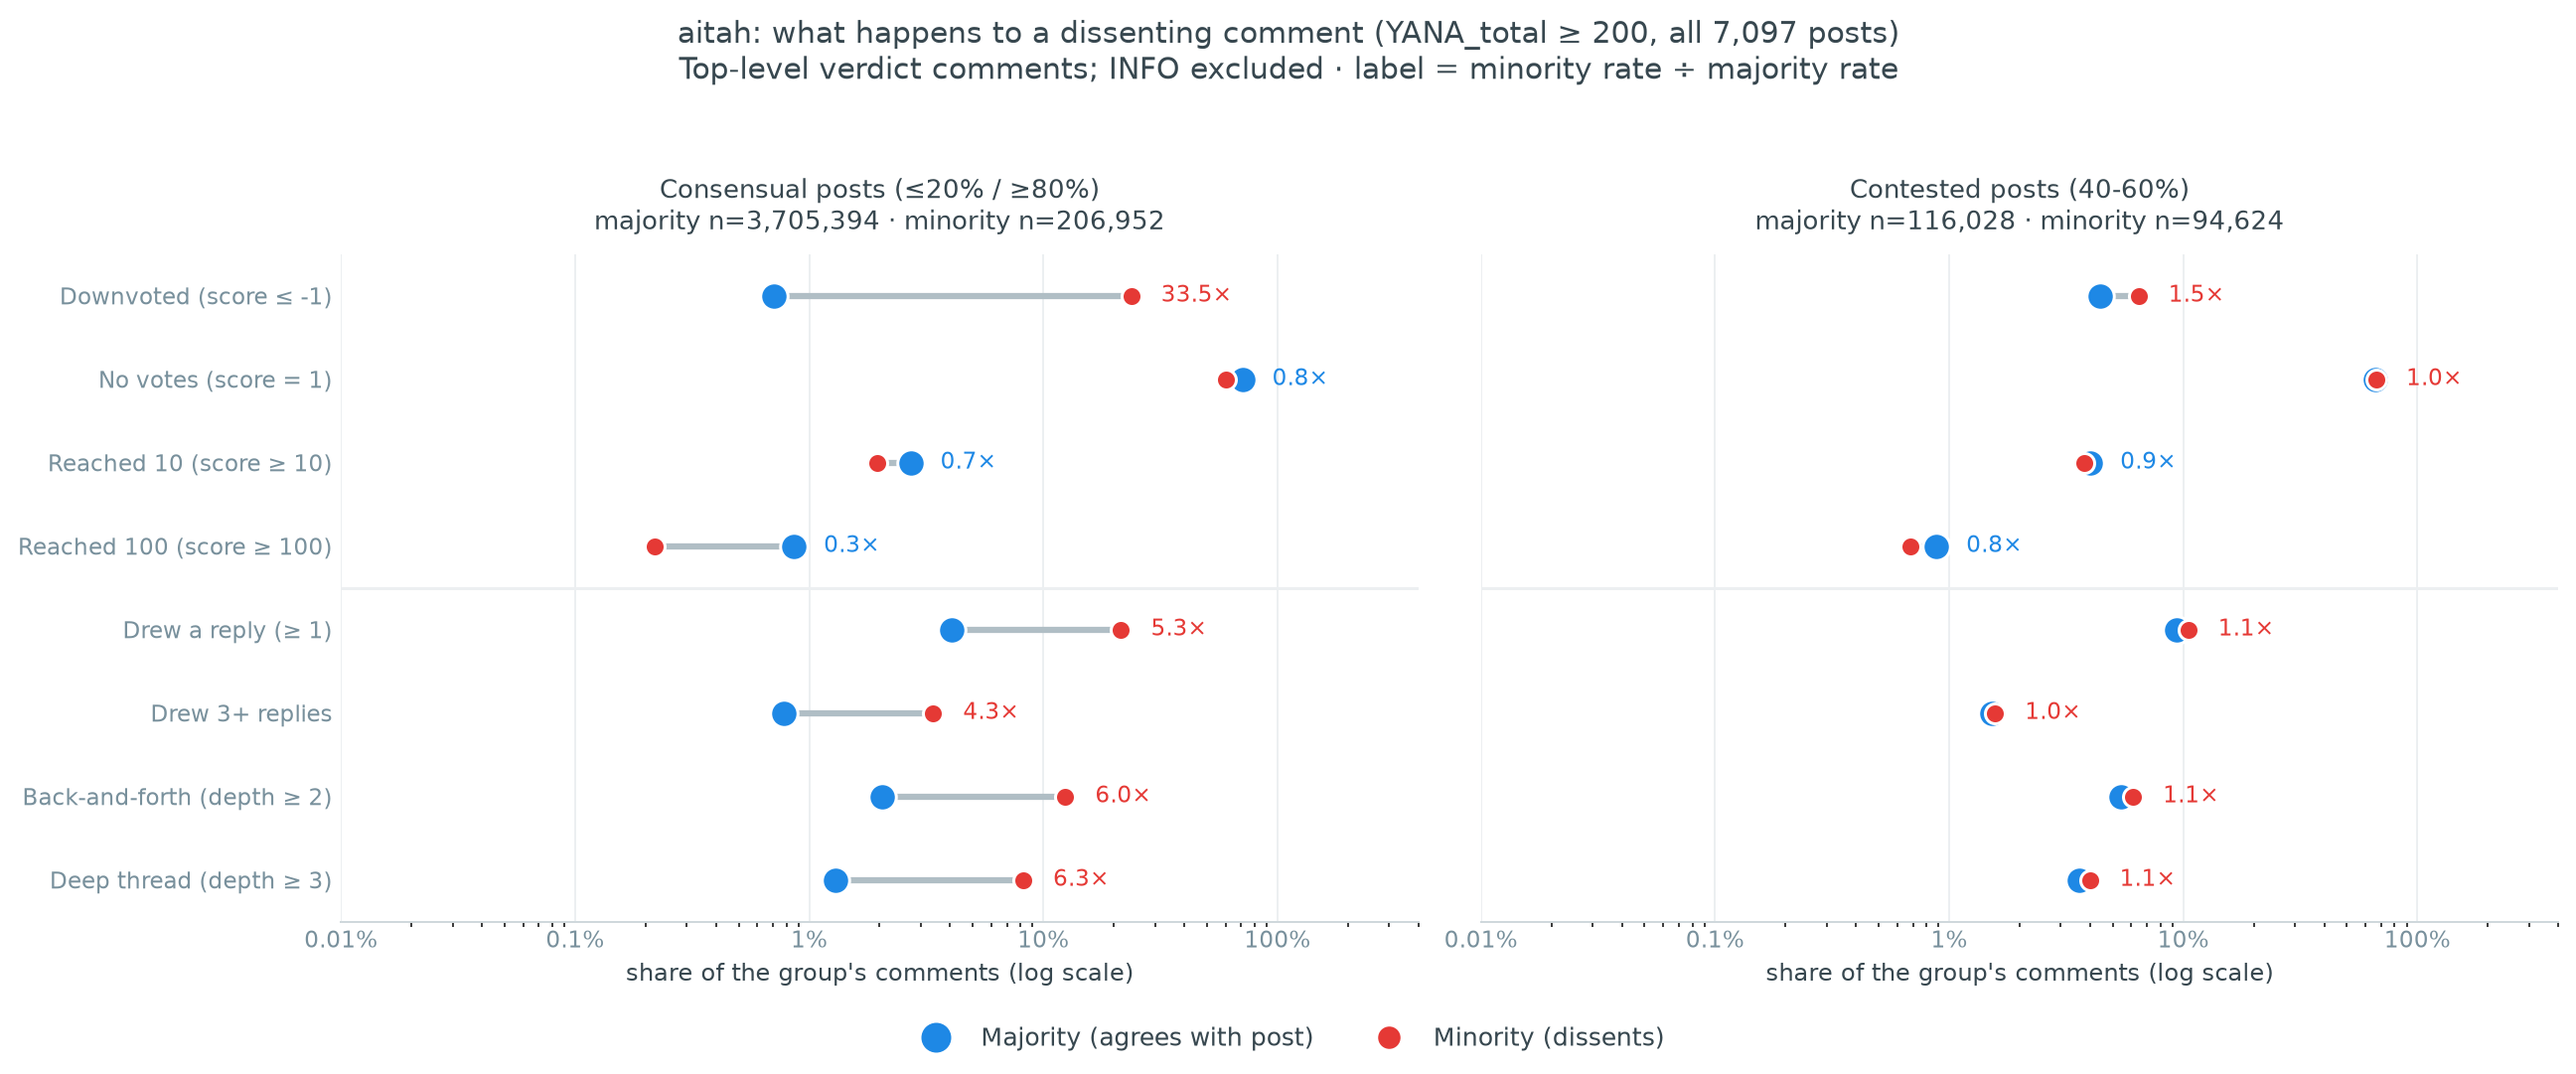
\includegraphics[width=\columnwidth]{figures/aitah_engagement_by_side.png}

    \caption{Comment scores and direct-reply counts by alignment and agreement level in AITA and AITAH. Posts satisfy $\mathrm{YANA\_total}\ge200$. This is the majority--minority baseline, not the matched-story analysis.}
    \label{fig:engagement-by-consensus}
\end{figure}

In the reply-tree sample, high-agreement AITA minority comments have a mean
depth of $0.82$, compared with $0.13$ for majority comments; $15.7\%$ versus
$2.5\%$ reach a depth of at least two
(Figure~\ref{fig:reply-depth-comparison}). The differences narrow in
low-agreement posts.

\textbf{[TODO: verify that the reception figures incorporate AITAH's
H-suffixed verdict aliases. Reconcile the full-data score/reply summaries
with the sampled figures and report the sample for each comparison.]}

\begin{figure}[t]
    \centering

    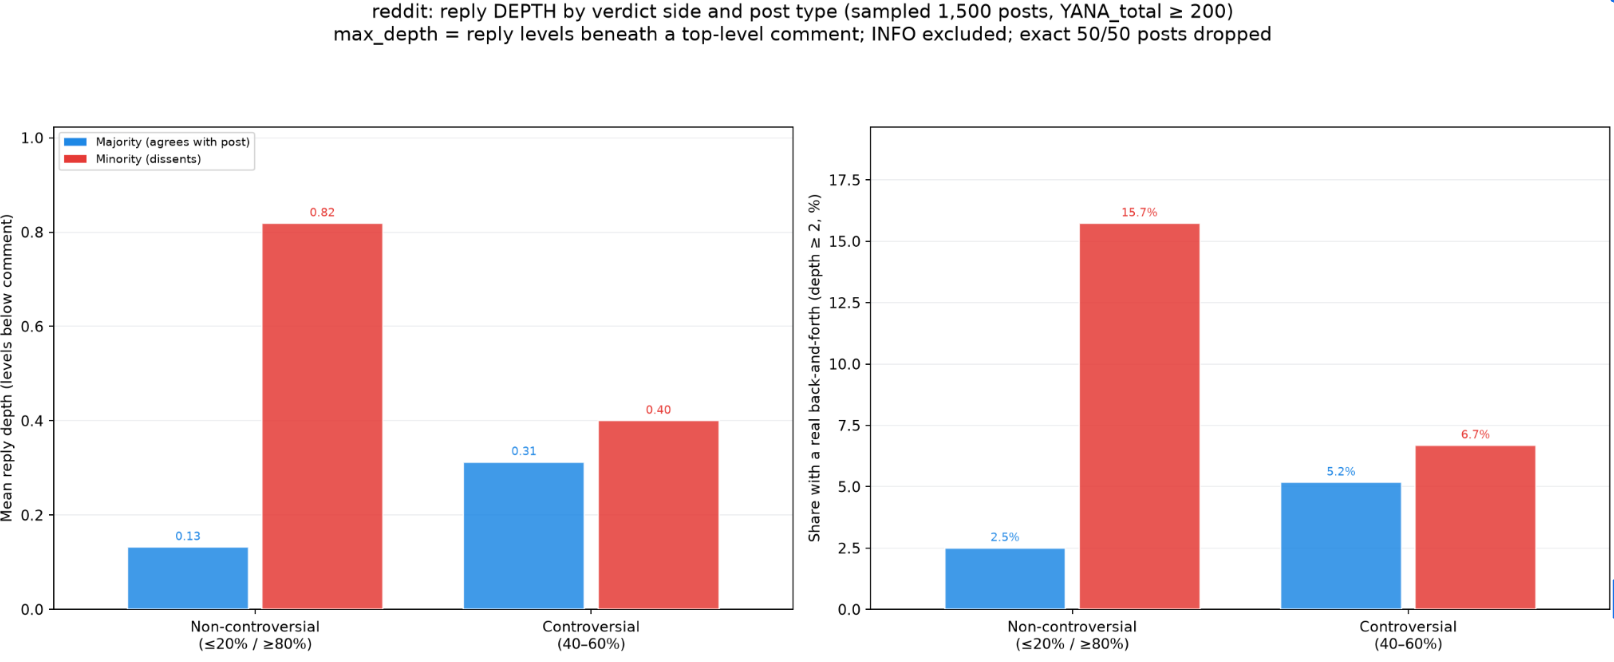
\includegraphics[width=\columnwidth]
    {figures/reply_depth_AITA.png}

    \vspace{0.5em}

    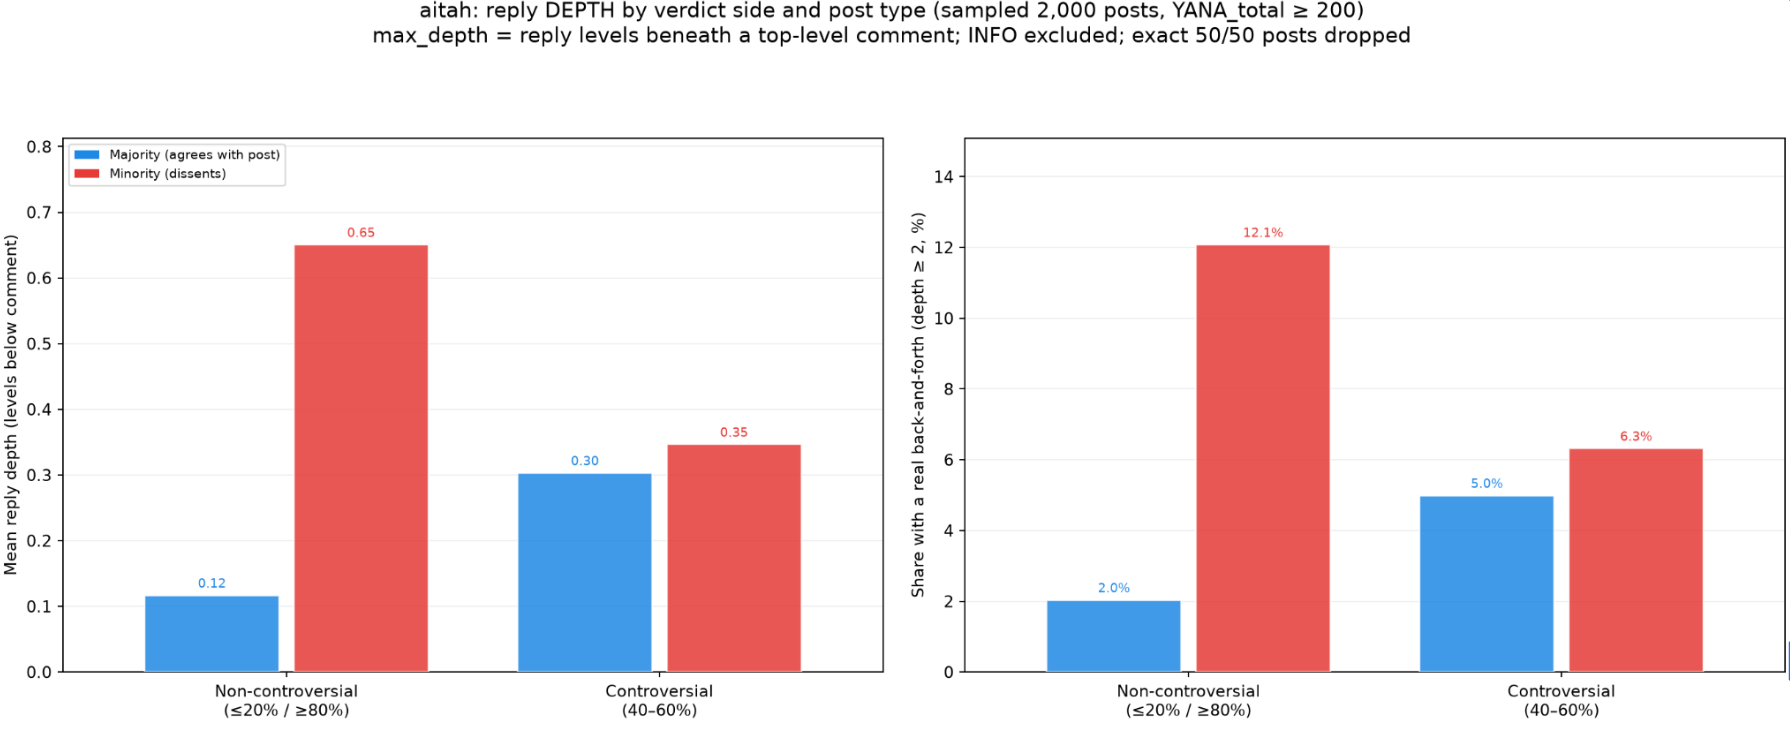
\includegraphics[width=\columnwidth]
    {figures/reply_depth_AITAH.png}

    \caption{\textbf{Minority judgments generate deeper reply threads.}
    Mean reply depth and the proportion of threads reaching a depth of at least two in AITA (top) and AITAH (bottom). Results compare majority- and minority-side comments across high-agreement and low-agreement posts with $\mathrm{YANA\_total} \geq 200$. INFO comments and exact 50/50 verdict ties are excluded. The majority--minority difference is largest in high-agreement posts and narrows substantially in low-agreement posts.}

    \label{fig:reply-depth-comparison}
\end{figure}

\subsection{RQ1: Reception of Blaming and Defending Dissent}
\label{subsec:res-direction}

\paragraph{Lower scores and more replies in both directions.}
Figure~\ref{fig:dissent-direction} separates blaming and defending dissent
in high-agreement posts, each with majority comments in the same dominant-
verdict context as a reference. In AITA, blaming minority comments have a
mean score of $-3.2$, versus $37.2$ for majority comments in NA-dominant
posts. Defending minority comments have a mean score of $-2.4$, versus
$35.4$ for majority comments in YA-dominant posts. Both directions therefore
reproduce the minority score disadvantage.

Replies show the opposite ordering. More than one direct reply is recorded
for $29.3\%$ of blaming minority comments and $17.2\%$ of defending minority
comments, compared with $4.6\%$ and $4.1\%$ of their respective majority
baselines. These percentages concern more than one reply, not receipt of
any reply. Blaming dissent has the lower mean score and a $1.70$-fold higher
rate of drawing more than one reply than defending dissent.

The existing depth summary reports that $17.8\%$ of blaming and $9.5\%$ of
defending minority comments seed subtrees deeper than two levels, a ratio
of $1.87$. \textbf{[TODO: verify whether this cutoff is depth greater than
2 or at least 2, supply the direction-specific depth figure or table, and
report the contributing post/comment counts and uncertainty.]}

\begin{figure}[t]
  \centering
  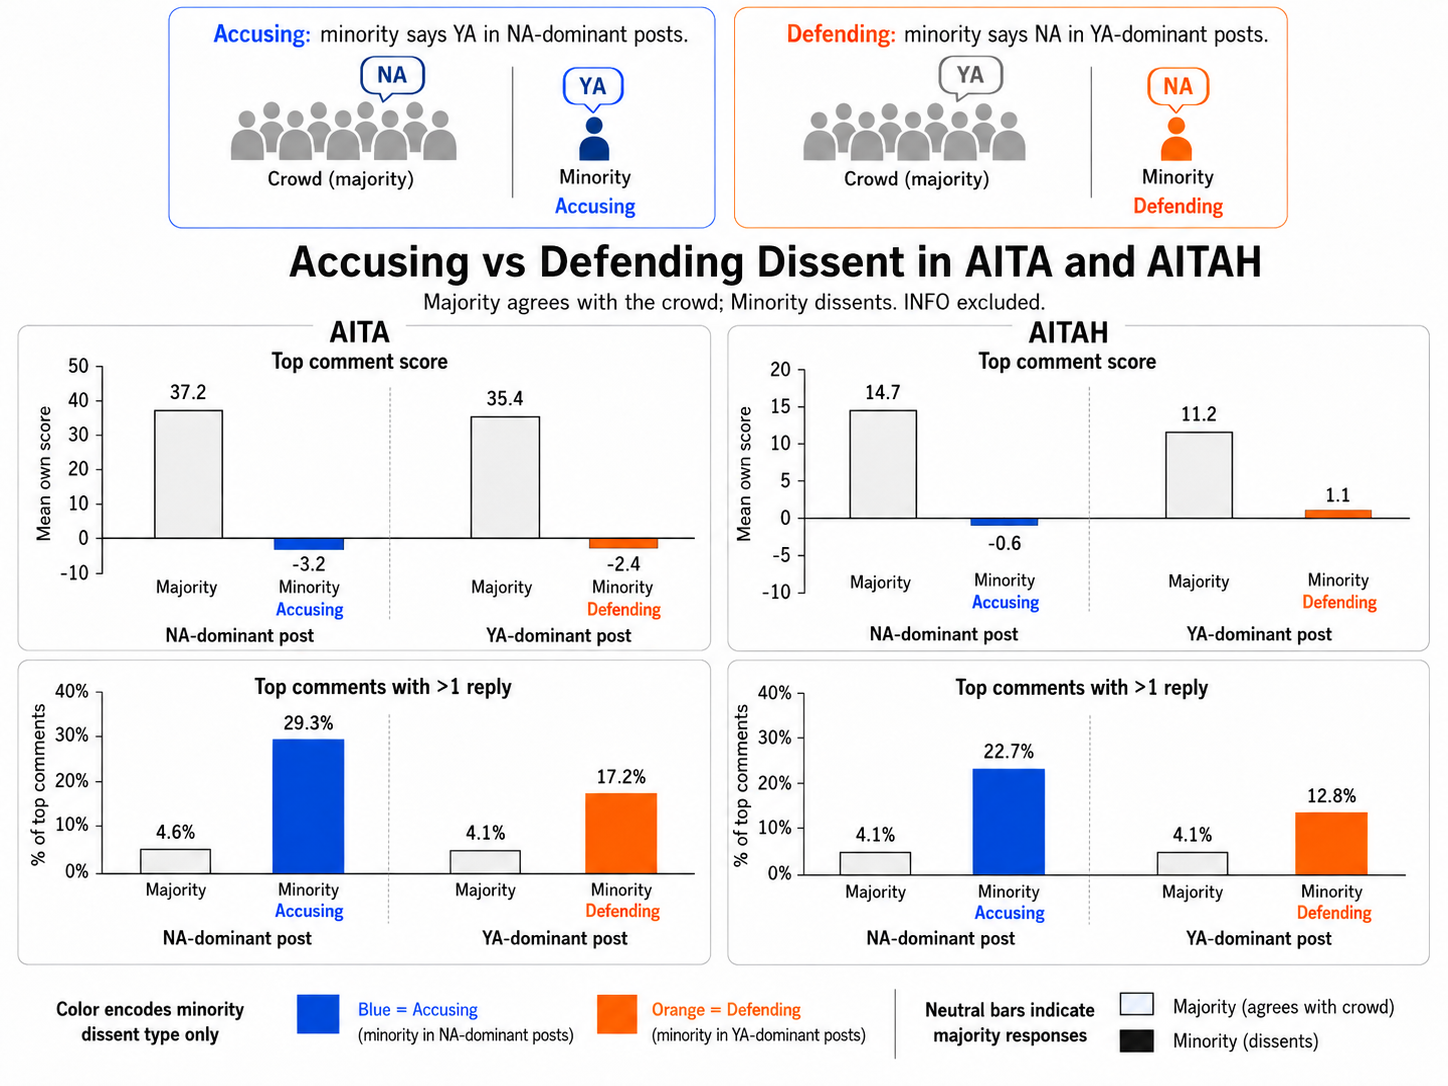
\includegraphics[width=\columnwidth]{figures/direction.png}
  \caption{Comment scores and the proportion of verdict comments receiving more than one direct reply, separately for blaming and defending dissent and their respective majority baselines. AITA is discussed in RQ1 and AITAH in RQ3. \textbf{[TODO: confirm whether the displayed score/reply values use all eligible comments or the previously reported 1,500-post sample per community; update the figure's ``Accusing'' labels to ``Blaming''.]}}
    \label{fig:dissent-direction}
\end{figure}

\paragraph{From reply volume to response type.}
\label{subsec:res-rq2}
The direct-response annotations, excluding OP participation, indicate higher
challenge proportions for minority than majority parent comments across the
analyzed community and agreement-tail strata. This comparison concerns the
composition of labeled replies rather than the probability of receiving a
reply. It therefore adds information about the responses accompanying the
minority reply advantage, without treating every reply as a challenge.

\textbf{[TODO: insert the response-type distribution figure and report
support, challenge, information-seeking, and other proportions, unique pair
counts, and uncertainty by stratum. Report blaming--defending contrasts
separately: the majority--minority challenge difference alone does not
establish which direction receives the higher challenge proportion.
Complete annotation validation before presenting these as final estimates.]}

\paragraph{Reception by comment arrival time.}
Among comments arriving during the first 18 hours, those posted in the first
hour have the highest mean scores and direct-reply counts
(Figure~\ref{fig:comment-engagement-over-time}). In high-agreement AITA
posts, the minority reply advantage is most pronounced among early comments
and becomes smaller for later arrivals. These are recorded reception outcomes
grouped by comment arrival hour, not repeated observations of a comment's
score or replies over its lifetime.

\begin{figure}[t]
    \centering

    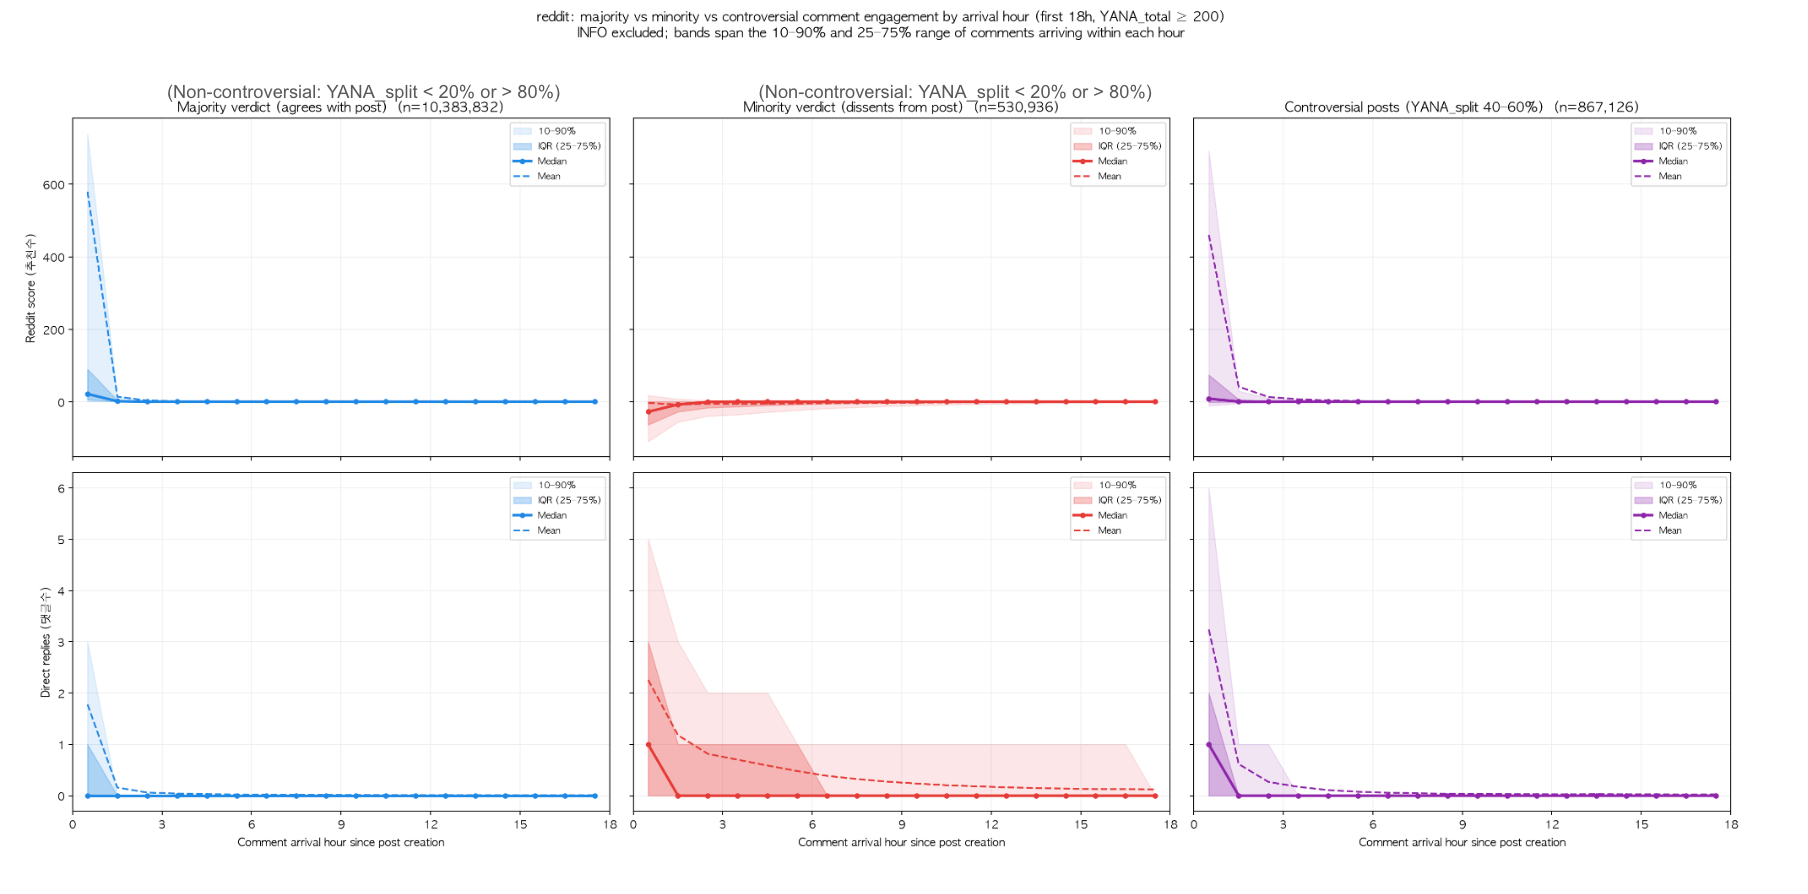
\includegraphics[width=\columnwidth]
    {figures/comment_engagement_aita.png}

    \vspace{0.5em}

    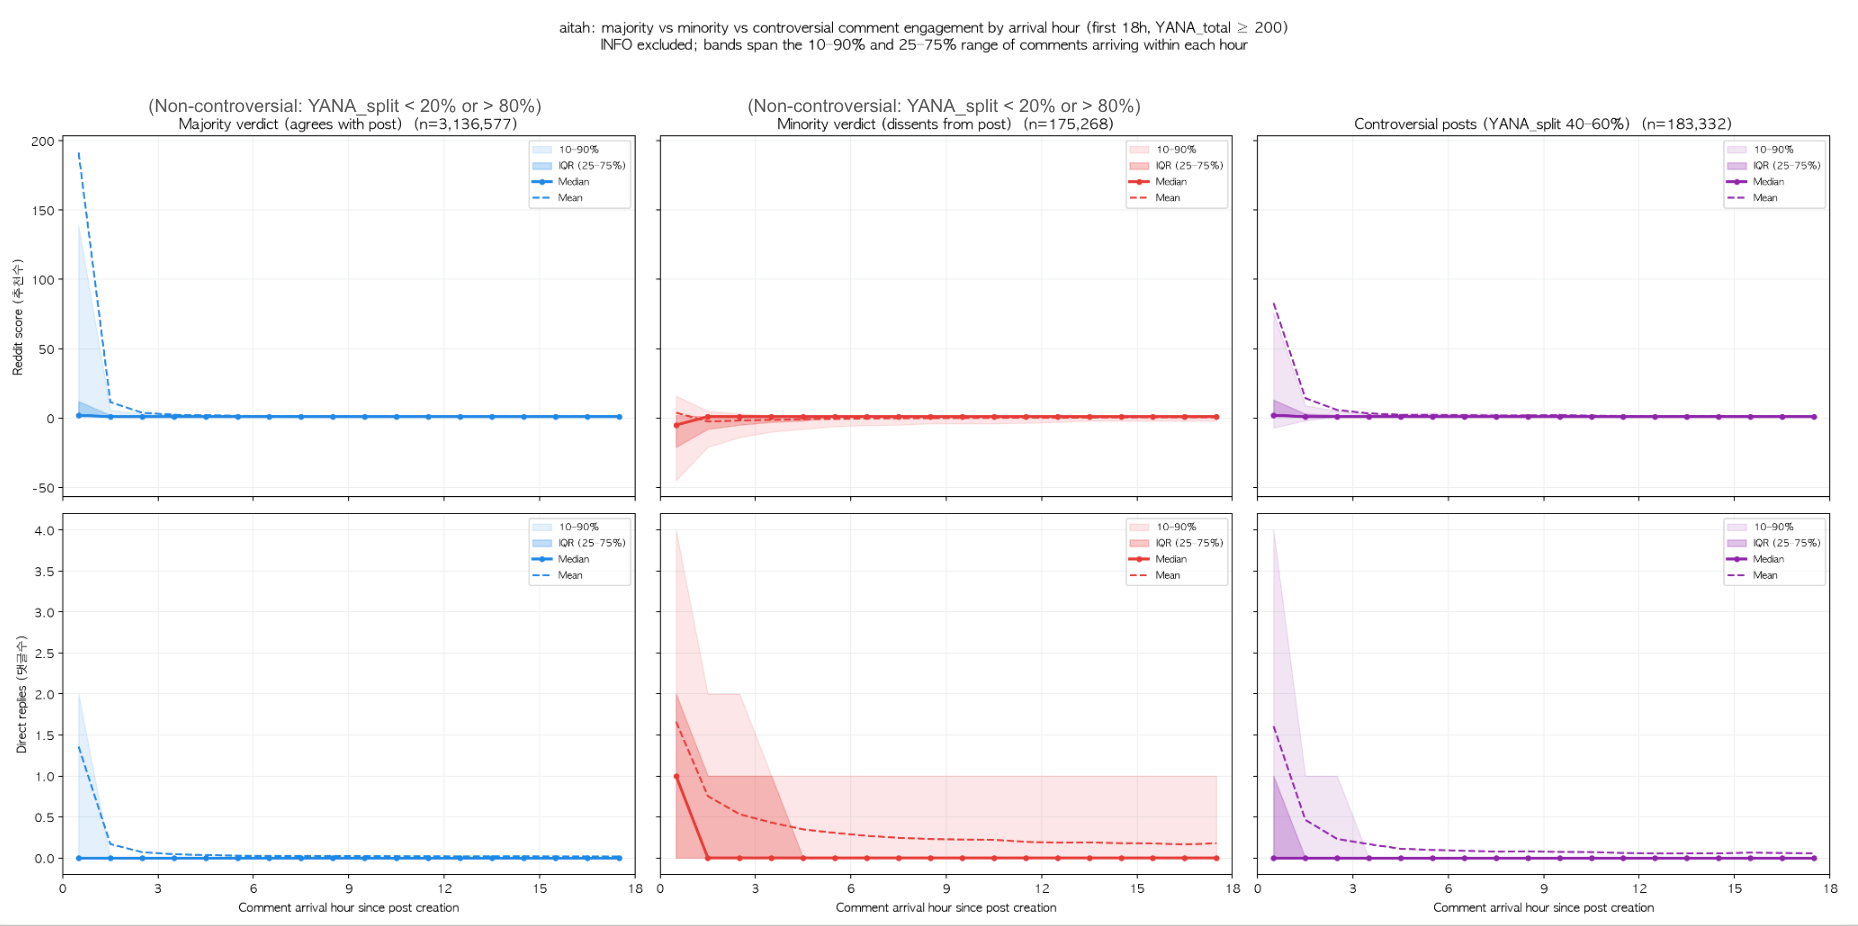
\includegraphics[width=\columnwidth]
    {figures/comment_engagement_aitah.png}

    \caption{\textbf{Comment engagement is concentrated in the earliest hours after submission.}
    Comment scores and direct replies by arrival hour for majority, minority,
    and comments in low-agreement posts in AITA (top) and AITAH (bottom).
    Lines show hourly means and medians, while shaded regions show the
    interquartile and 10th--90th percentile ranges. Analyses are restricted to
    the first 18 hours and posts with $\mathrm{YANA\_total} \geq 200$; INFO
    comments are excluded.}

    \label{fig:comment-engagement-over-time}
\end{figure}

\subsection{RQ2: Prevalence of Blaming and Defending Dissent Over Time}
\label{subsec:res-temporal}

This analysis concerns how prevalent each direction of dissent is among
observed verdict comments, separately from how confidently those judgments
are expressed. The participation data are not restricted to the
certainty-annotated sample.

\paragraph{Cumulative minority share.}
The existing cumulative-share figure shows an early decline followed by a
recovery in AITA for both dissent directions. After the initial hours,
defending share rises gradually, while blaming share levels off
(Figure~\ref{fig:minority-ratio-time}). These cumulative curves are distinct
from the window-specific measure defined in Section~\ref{subsec:method-temporal}.

\begin{figure}[t]
    \centering
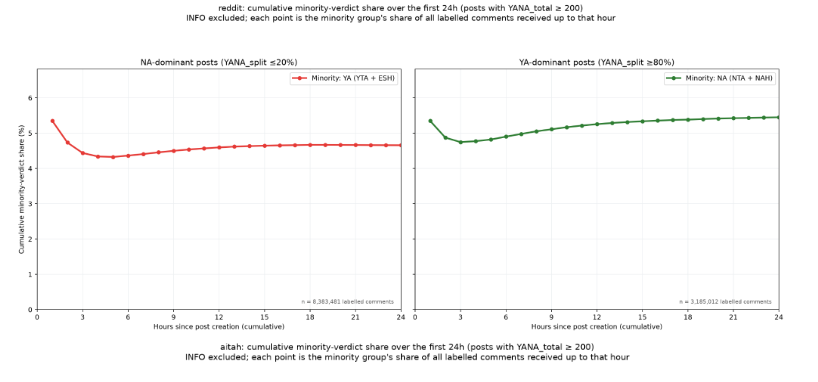
\includegraphics[width=\columnwidth]
    {figures/aita_minority_verdict_ratio.png}

    \vspace{0.5em}

    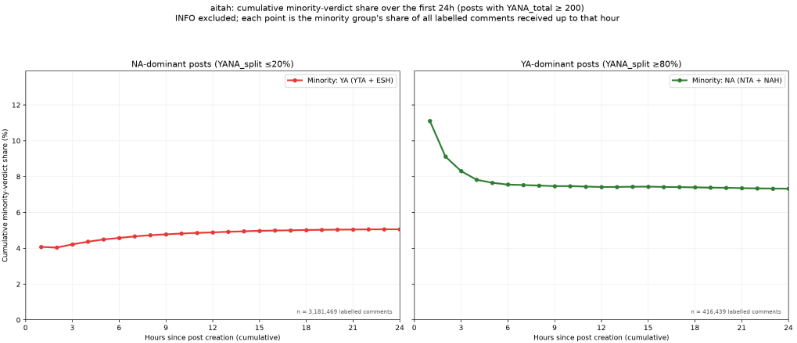
\includegraphics[width=\columnwidth]
    {figures/aitah_minority_verdict_ratio.png}

    \caption{Cumulative minority-verdict shares during the first 24 hours in high-agreement AITA (top) and AITAH (bottom) posts with at least 200 verdicts. Blaming share is calculated within NA-dominant posts and defending share within YA-dominant posts. These curves include comments up to each time point, unlike window-specific minority shares.}
    \label{fig:minority-ratio-time}
\end{figure}

\textbf{[TODO: verify the share figure's aggregation and contributing counts;
add window-specific estimates and the low-agreement comparison with
uncertainty. The existing figure covers only the first 24 hours and does
not establish the full observed trajectory. Do not substitute results from
the certainty-annotated sample for full-data participation estimates.]}

\subsection{RQ3: Extension to AITAH}
\label{subsec:res-community}

\paragraph{Shared reception ordering, different magnitudes.}
AITAH reproduces the baseline score--reply pattern. In high-agreement posts,
majority and minority comments have mean scores of $14.30$ and $-0.19$,
and mean direct-reply counts of $0.12$ and $0.38$, respectively
(Figure~\ref{fig:engagement-by-consensus}). In low-agreement posts, both
sides average $0.21$ replies. Mean reply depths in the high-agreement
reply-tree sample are $0.12$ for majority and $0.65$ for minority comments;
$2.0\%$ and $12.1\%$ reach depth two or more
(Figure~\ref{fig:reply-depth-comparison}).

The directional comparison also recurs (Figure~\ref{fig:dissent-direction}).
Blaming minority comments average $-0.6$, versus $14.7$ for their majority
baseline; defending minority comments average $1.1$, versus $11.2$.
The proportions receiving more than one reply are $22.7\%$ for blaming and
$12.8\%$ for defending, against $4.1\%$ for each majority baseline.
The blaming-to-defending reply ratio is $1.77$, compared with $1.70$ in AITA.
The reported depth-threshold rates are $13.2\%$ and $7.2\%$ (ratio $1.83$),
subject to the cutoff verification noted under RQ1. Thus, the directional
ordering is shared, although the raw score gaps and reply rates differ.
\textbf{[TODO: report uncertainty for between-community contrasts and confirm
that all direct comparisons use the common calendar period.]}

\paragraph{Different patterns of minority participation.}
The existing full-data cumulative curves show declining defending share in
AITAH, from approximately $11\%$ to $7\%$
(Figure~\ref{fig:minority-ratio-time}).
\textbf{[TODO: update the directional window-specific share figures,
with contributing counts, low-agreement comparisons, and intervals. Do not attribute
community differences to the 18-hour rule.]}

\paragraph{Illustrative cross-posted stories.}
\label{subsec:res-duplicates}
\textbf{[TODO: add a small number of verified examples showing how the same
story is received in the two communities. Explain case selection and show
relevant judgments or exchanges. These examples illustrate the comparison;
they are not a matched-sample test of institutional effects. The earlier
quantitative duplicate-post draft is retained in the non-compiled notes file,
not used as a principal result.]}

\subsection{Supplementary Analysis: Expressed Certainty}
\label{subsec:res-certainty-contrasts}

Separately from temporal prevalence, the annotated sample characterizes
how confidently blaming and defending dissent are expressed over the full
observed period. In high-agreement AITA posts, the mean within-post
certainty-$4$ proportion is $66.1\%$ for blaming and $58.1\%$ for defending,
a difference of $8.0$ percentage points ($95\%$ post-bootstrap CI
$[3.9,12.2]$); the low-agreement contrast remains uncertain.
These are descriptive differences between post cohorts, not evidence of
certainty increasing over time. Full distributions and additional contrasts
appear in Appendix~\ref{sec:appendix-certainty-comparison}
(Figure~\ref{fig:certainty-low-high}), alongside annotation-version caution
and the small AITAH high-agreement defending cohort ($15$ posts).
\textbf{[TODO: complete annotation validation before finalizing these results.]}
